%%%%%%%%%%%%%%%%%%%%%%%%%%%%%%%%%%%%%%%%%%%%%%%%%%%%%%%%%%%
%% Capítulo 9 — Resultados del estudio 
%%%%%%%%%%%%%%%%%%%%%%%%%%%%%%%%%%%%%%%%%%%%%%%%%%%%%%%%%%%

\chapter{Resultados del estudio}\label{cap:resultados}

Este capítulo presenta los resultados obtenidos en el estudio de validación descrito en el capítulo~\ref{cap:validacion}. El análisis se organiza en torno a los tres constructos del modelo TAM, utilidad percibida (PU), facilidad de uso percibida (PEOU) e intención de uso (ITU), y se complementa con la valoración de funcionalidades específicas recogida en el Bloque~E y con el análisis cualitativo de las preguntas abiertas. La muestra final está compuesta por $n = 11$ participantes que completaron el cuestionario entre el 22 de julio y el 26 de agosto de 2026, coincidiendo con el período de evaluación del sistema descrito en el capítulo~\ref{cap:ejecucion}.

%%%%%%%%%%%%%%%%%%%%%%%%%%%%%%%%%%%%%%%%%%%%%%%%%%%%%%%%%%%
\section{Perfil de la muestra}\label{sec:perfil-muestra}
%%%%%%%%%%%%%%%%%%%%%%%%%%%%%%%%%%%%%%%%%%%%%%%%%%%%%%%%%%%

La tabla~\ref{tab:demografia} resume las características demográficas y de experiencia previa de los once participantes (variables del Bloque~A del cuestionario).

\begin{table}[h!]
\centering
\caption{Perfil demográfico y de experiencia de los participantes ($n = 11$).}
\label{tab:demografia}
\begin{tabular}{@{} p{9.5cm} r @{}}
\hline
\rule{0pt}{10pt}\textbf{Característica / Categoría} & \textbf{$n$ (\%)} \\
\hline
\rule{0pt}{12pt}\textbf{Edad} & \\
\quad 20--24 años & 8 (72{,}7\,\%) \\
\quad 25--29 años & 3 (27{,}3\,\%) \\[2pt]
\hline
\rule{0pt}{12pt}\textbf{Género} & \\
\quad Hombre & 8 (72{,}7\,\%) \\
\quad Mujer  & 3 (27{,}3\,\%) \\[2pt]
\hline
\rule{0pt}{12pt}\textbf{Nivel de estudios} & \\
\quad Máster & 9 (81{,}8\,\%) \\
\quad Grado  & 2 (18{,}2\,\%) \\[2pt]
\hline
\rule{0pt}{12pt}\textbf{Conocimiento previo de BPMN} (escala 1--7) & \\
\quad 3 --- básico & 2 (18{,}2\,\%) \\
\quad 4 --- medio  & 8 (72{,}7\,\%) \\
\quad 5 --- alto   & 1 (9{,}1\,\%) \\[2pt]
\hline
\rule{0pt}{12pt}\textbf{Experiencia con herramientas de modelado} (escala 1--7) & \\
\quad 2 --- escasa & 1 (9{,}1\,\%) \\
\quad 3 --- baja   & 1 (9{,}1\,\%) \\
\quad 4 --- media  & 6 (54{,}5\,\%) \\
\quad 5 --- alta   & 3 (27{,}3\,\%) \\[2pt]
\hline
\rule{0pt}{12pt}\textbf{Frecuencia de uso de IA generativa} & \\
\quad Habitual (varias veces/semana) & 4 (36{,}4\,\%) \\
\quad Diaria                         & 7 (63{,}6\,\%) \\
\hline
\end{tabular}
\end{table}

El perfil dominante es el de un estudiante de máster joven (20--24 años), con un conocimiento medio de BPMN (nivel 4 en el 72{,}7\,\%) y una experiencia fluida tanto con herramientas de modelado como con sistemas de IA generativa. Este perfil es coherente con el tipo de usuario objetivo de la herramienta (profesionales técnicos que modelan procesos de negocio), aunque el rango de experiencia previa con IA (entre \textit{habitual} y \textit{diaria}) sugiere una muestra sensiblemente familiarizada con este tipo de tecnologías, lo que puede influir positivamente en la percepción de la facilidad de uso.

%%%%%%%%%%%%%%%%%%%%%%%%%%%%%%%%%%%%%%%%%%%%%%%%%%%%%%%%%%%
\section{Fiabilidad de las escalas}\label{sec:fiabilidad}
%%%%%%%%%%%%%%%%%%%%%%%%%%%%%%%%%%%%%%%%%%%%%%%%%%%%%%%%%%%

Antes de proceder al análisis por constructo se estimó la consistencia interna de cada escala mediante el coeficiente alfa de Cronbach ($\alpha$). Para una muestra piloto de $n = 11$, un valor $\alpha \geq 0{,}70$ se considera aceptable en la literatura de validación de instrumentos psicométricos. Las figuras~\ref{fig:alpha-pu}, \ref{fig:alpha-peou} y \ref{fig:alpha-itu} muestran el desarrollo numérico del cálculo para cada constructo; la tabla~\ref{tab:alpha} resume los resultados.

%%--- Figura: cálculo alfa de Cronbach para PU ---
\begin{figure}[h!]
\centering
\[
  \alpha_{\mathrm{PU}}
  = \frac{k}{k-1}\!\left(1 - \frac{\displaystyle\sum_{i=1}^{k}\sigma_i^2}{\sigma_{\mathrm{total}}^2}\right)
  = \frac{11}{10}\!\left(1 - \frac{7{,}33}{35{,}29}\right)
  = 1{,}1 \times \bigl(1 - 0{,}208\bigr)
  = 1{,}1 \times 0{,}792
  \approx \mathbf{0{,}87}
\]
\caption{Cálculo del alfa de Cronbach para la escala PU ($k = 11$ ítems, $n = 11$).
  $\sum\sigma_i^2 = 7{,}33$ es la suma de las varianzas individuales de cada ítem;
  $\sigma_{\mathrm{total}}^2 = 35{,}29$ es la varianza de la puntuación total del constructo.}
\label{fig:alpha-pu}
\end{figure}

%%--- Figura: cálculo alfa de Cronbach para PEOU ---
\begin{figure}[h!]
\centering
\[
  \alpha_{\mathrm{PEOU}}
  = \frac{k}{k-1}\!\left(1 - \frac{\displaystyle\sum_{i=1}^{k}\sigma_i^2}{\sigma_{\mathrm{total}}^2}\right)
  = \frac{12}{11}\!\left(1 - \frac{12{,}32}{60{,}84}\right)
  = 1{,}091 \times \bigl(1 - 0{,}202\bigr)
  = 1{,}091 \times 0{,}798
  \approx \mathbf{0{,}87}
\]
\caption{Cálculo del alfa de Cronbach para la escala PEOU ($k = 12$ ítems, $n = 11$).
  $\sum\sigma_i^2 = 12{,}32$;
  $\sigma_{\mathrm{total}}^2 = 60{,}84$.}
\label{fig:alpha-peou}
\end{figure}

%%--- Figura: cálculo alfa de Cronbach para ITU ---
\begin{figure}[h!]
\centering
\[
  \alpha_{\mathrm{ITU}}
  = \frac{k}{k-1}\!\left(1 - \frac{\displaystyle\sum_{i=1}^{k}\sigma_i^2}{\sigma_{\mathrm{total}}^2}\right)
  = \frac{5}{4}\!\left(1 - \frac{7{,}80}{25{,}65}\right)
  = 1{,}250 \times \bigl(1 - 0{,}304\bigr)
  = 1{,}250 \times 0{,}696
  \approx \mathbf{0{,}87}
\]
\caption{Cálculo del alfa de Cronbach para la escala ITU ($k = 5$ ítems, $n = 11$).
  $\sum\sigma_i^2 = 7{,}80$;
  $\sigma_{\mathrm{total}}^2 = 25{,}65$.}
\label{fig:alpha-itu}
\end{figure}

\begin{table}[h!]
\centering
\caption{Consistencia interna de las escalas TAM ($n = 10$).}
\label{tab:alpha}
\begin{tabular}{@{} l c c c @{}}
\hline
\rule{0pt}{10pt}\textbf{Constructo} & \textbf{Ítems} & $\bm{\alpha}$ & \textbf{Valoración} \\
\hline
\rule{0pt}{10pt}Utilidad percibida (PU)         & 11 & 0{,}87 & Buena \\
Facilidad de uso percibida (PEOU) & 12 & 0{,}87 & Buena \\
Intención de uso (ITU)            &  5 & 0{,}87 & Buena \\
\hline
\end{tabular}
\end{table}

Los tres constructos presentan $\alpha = 0{,}87$, superando con holgura el umbral de $0{,}70$ y situándose en el rango «bueno» ($0{,}80$--$0{,}90$). Estos resultados indican que los ítems de cada bloque miden de forma consistente la misma dimensión latente, lo que legitima la construcción de una puntuación compuesta por constructo a partir de la media de sus ítems.

La figura~\ref{fig:radar-tam} ofrece una visión global de las puntuaciones compuestas de los cuatro bloques del cuestionario, mostrando cómo los constructos TAM (PU, PEOU e ITU) se sitúan todos por encima de 5{,}7 sobre 7, con PU y PEOU próximos a 6{,}2, lo que indica una percepción muy positiva de la herramienta en su conjunto.

\begin{figure}[h!]
\centering
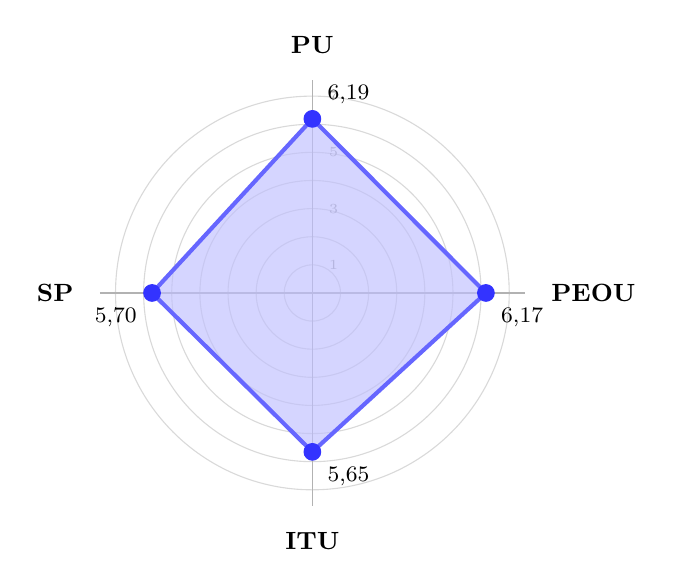
\begin{tikzpicture}
  % Circles at each integer 1-7, max radius 2.5cm
  \foreach \v in {1,2,3,4,5,6,7}{
    \pgfmathsetmacro{\rr}{\v/7*2.5}
    \draw[gray!30, thin] (0,0) circle (\rr cm);
  }
  % Tick labels on top axis (right side to avoid overlap)
  \foreach \v/\lbl in {1/1, 3/3, 5/5, 7/7}{
    \pgfmathsetmacro{\rr}{\v/7*2.5}
    \node[right=1pt, font=\tiny, gray!70] at (0.05,\rr) {\lbl};
  }
  % Axis lines
  \draw[gray!60] (0,-2.7) -- (0,2.7);
  \draw[gray!60] (-2.7,0) -- (2.7,0);
  % Data polygon:
  %   PU(top)=6.19   → r = 6.19/7*2.5 = 2.211
  %   PEOU(right)=6.17 → r = 6.17/7*2.5 = 2.204
  %   ITU(bottom)=5.65 → r = 5.65/7*2.5 = 2.018
  %   SP(left)=5.70  → r = 5.70/7*2.5 = 2.036
  \fill[blue!25, opacity=0.65]
    (0,2.211) -- (2.204,0) -- (0,-2.018) -- (-2.036,0) -- cycle;
  \draw[blue!60, line width=1.5pt]
    (0,2.211) -- (2.204,0) -- (0,-2.018) -- (-2.036,0) -- cycle;
  % Data points
  \filldraw[blue!80] (0,2.211)  circle (3pt);
  \filldraw[blue!80] (2.204,0)  circle (3pt);
  \filldraw[blue!80] (0,-2.018) circle (3pt);
  \filldraw[blue!80] (-2.036,0) circle (3pt);
  % Axis name labels
  \node[above=6pt, font=\small\bfseries] at (0,2.7)   {PU};
  \node[right=6pt, font=\small\bfseries] at (2.7,0)   {PEOU};
  \node[below=6pt, font=\small\bfseries] at (0,-2.7)  {ITU};
  \node[left=6pt,  font=\small\bfseries] at (-2.7,0)  {SP};
  % Score value labels
  \node[above right=2pt, font=\footnotesize] at (0,2.211)  {6{,}19};
  \node[below right=2pt, font=\footnotesize] at (2.204,0)  {6{,}17};
  \node[below right=2pt, font=\footnotesize] at (0,-2.018) {5{,}65};
  \node[below left=2pt,  font=\footnotesize] at (-2.036,0) {5{,}70};
\end{tikzpicture}
\caption{Puntuaciones compuestas por constructo TAM ($n=11$; escala 1--7). La distancia al centro es proporcional a la puntuación media del constructo.}
\label{fig:radar-tam}
\end{figure}

%%%%%%%%%%%%%%%%%%%%%%%%%%%%%%%%%%%%%%%%%%%%%%%%%%%%%%%%%%%
\section{Utilidad percibida}\label{sec:resultados-pu}
%%%%%%%%%%%%%%%%%%%%%%%%%%%%%%%%%%%%%%%%%%%%%%%%%%%%%%%%%%%

La puntuación compuesta de utilidad percibida (PU) se calculó como la media aritmética de los once ítems del Bloque~B para cada participante. La media global obtenida fue $\bar{x}_{\text{PU}} = 6{,}19$ ($SD = 0{,}57$; escala de 1 a 7), lo que equivale a un $88{,}4$\,\% de la puntuación máxima posible. La tabla~\ref{tab:puItems} detalla la media por ítem.

\begin{table}[H]
\centering
\caption{Medias por ítem del Bloque~B (Utilidad percibida, $n = 11$; escala 1--7).}
\label{tab:puItems}
\begin{tabular}{@{} c p{9.5cm} c @{}}
\hline
\rule{0pt}{10pt}\textbf{Ítem} & \textbf{Enunciado resumido} & $\bar{x}$ \\
\hline
\rule{0pt}{10pt}PU1  & El sistema permite crear diagramas BPMN más rápido que herramientas tradicionales & 6{,}73 \\
PU2  & El uso del sistema mejora la productividad en el modelado de procesos & 6{,}09 \\
PU3  & El sistema es útil para procesos con varios departamentos y actores externos & 6{,}36 \\
PU4  & El sistema identifica correctamente los participantes del proceso & 6{,}55 \\
PU5  & Las bifurcaciones propuestas reflejan adecuadamente la lógica del proceso & 5{,}73 \\
PU6  & Las preguntas del sistema durante la generación guiada son pertinentes & 6{,}18 \\
PU7  & La colaboración paso a paso produce un diagrama más fiel que la generación autónoma & 5{,}82 \\
PU8  & La edición conversacional permite ajustar el diagrama sin conocer la sintaxis BPMN & 5{,}91 \\
PU9  & El análisis PERVAL integrado ayuda a identificar qué elementos aportan más valor & 5{,}55 \\
PU10 & El modo de generación completa es útil para obtener rápidamente un primer borrador & 6{,}64 \\
PU11 & En general, el sistema es una herramienta valiosa para el modelado de procesos & 6{,}55 \\
\hline
\multicolumn{2}{@{}l}{\rule{0pt}{10pt}\textbf{Puntuación compuesta PU}} & \textbf{6{,}19} \\
\hline
\end{tabular}
\end{table}

Los ítems con media más alta corresponden a la velocidad de creación de diagramas (PU1 $= 6{,}73$, $Mdn=7$, $Mo=7$), al modo de generación completa (PU10 $= 6{,}64$) y al juicio global de valor (PU11 $= 6{,}55$). El ítem de menor puntuación es PU9, relativo al análisis PERVAL ($\bar{x} = 5{,}55$), lo que sugiere que los participantes valoran la característica pero perciben un margen de mejora respecto a su integración en el flujo de trabajo. El ítem PU7 (colaboración paso a paso frente a generación autónoma, $\bar{x} = 5{,}82$) registra un descenso respecto a la medición anterior, influido por la valoración de P11, que prefirió la generación completa como punto de partida.

La figura~\ref{fig:barchart-pu} muestra la distribución de respuestas para los ítems extremos del bloque: PU1 concentra el $72{,}7$\,\% de respuestas en el valor máximo 7 ($n=8$), mientras PU9 presenta una distribución más dispersa centrada en los valores 5 y 6.

\begin{figure}[H]
\centering
\begin{minipage}[t]{0.47\linewidth}
\centering
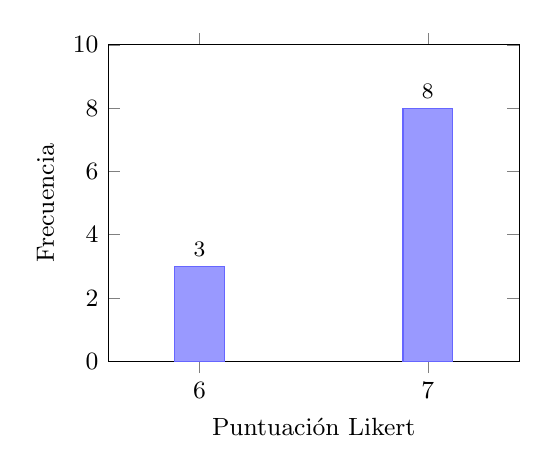
\begin{tikzpicture}
\begin{axis}[
  ybar, bar width=18pt,
  xlabel={Puntuación Likert},
  ylabel={Frecuencia},
  xtick=data,
  ytick={0,2,4,6,8,10},
  ymin=0, ymax=10,
  width=6.8cm, height=5.6cm,
  nodes near coords,
  every node near coord/.append style={font=\footnotesize},
  enlarge x limits=0.4,
  fill=blue!40,
  tick label style={font=\small},
  label style={font=\small},
]
\addplot[fill=blue!40, draw=blue!60] coordinates {(6,3) (7,8)};
\end{axis}
\end{tikzpicture}
\par\vspace{4pt}
{\small\textbf{PU1} — Velocidad de creación\par $\bar{x}=6{,}73$;\; $Mdn=7$;\; $Mo=7$}
\end{minipage}
\hfill
\begin{minipage}[t]{0.47\linewidth}
\centering
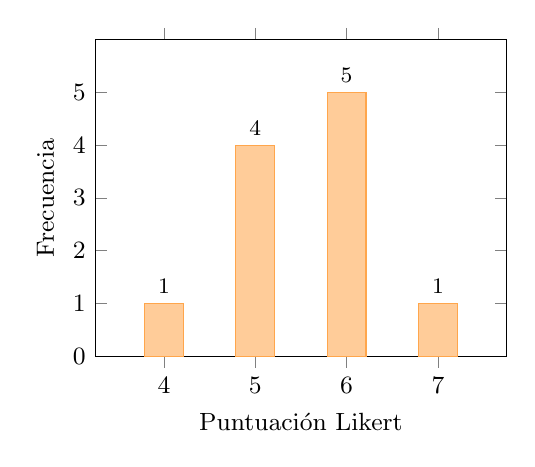
\begin{tikzpicture}
\begin{axis}[
  ybar, bar width=14pt,
  xlabel={Puntuación Likert},
  ylabel={Frecuencia},
  xtick=data,
  ytick={0,1,2,3,4,5},
  ymin=0, ymax=6,
  width=6.8cm, height=5.6cm,
  nodes near coords,
  every node near coord/.append style={font=\footnotesize},
  enlarge x limits=0.25,
  fill=orange!40,
  tick label style={font=\small},
  label style={font=\small},
]
\addplot[fill=orange!40, draw=orange!70] coordinates {(4,1) (5,4) (6,5) (7,1)};
\end{axis}
\end{tikzpicture}
\par\vspace{4pt}
{\small\textbf{PU9} — Análisis PERVAL\par $\bar{x}=5{,}55$;\; $Mdn=6$;\; $Mo=6$}
\end{minipage}
\caption{Distribución de respuestas para los ítems extremos del Bloque B ($n=11$): ítem de mayor puntuación (PU1) e ítem de menor puntuación (PU9).}
\label{fig:barchart-pu}
\end{figure}

%%%%%%%%%%%%%%%%%%%%%%%%%%%%%%%%%%%%%%%%%%%%%%%%%%%%%%%%%%%
\section{Facilidad de uso percibida}\label{sec:resultados-peou}
%%%%%%%%%%%%%%%%%%%%%%%%%%%%%%%%%%%%%%%%%%%%%%%%%%%%%%%%%%%

La media compuesta de facilidad de uso percibida (PEOU) fue $\bar{x}_{\text{PEOU}} = 6{,}17$ ($SD = 0{,}70$), equivalente al $88{,}1$\,\% de la puntuación máxima. La tabla~\ref{tab:peouItems} presenta las medias por ítem.

\begin{table}[H]
\centering
\caption{Medias por ítem del Bloque~C (Facilidad de uso percibida, $n = 11$; escala 1--7).}
\label{tab:peouItems}
\begin{tabular}{@{} c p{9.5cm} c @{}}
\hline
\rule{0pt}{10pt}\textbf{Ítem} & \textbf{Enunciado resumido} & $\bar{x}$ \\
\hline
\rule{0pt}{10pt}PEOU1  & Aprender a utilizar el sistema ha sido sencillo & 6{,}64 \\
PEOU2  & Describir el proceso en lenguaje natural es intuitivo & 6{,}27 \\
PEOU3  & La interfaz (editor BPMN y panel conversacional) es clara & 5{,}64 \\
PEOU4  & El número de preguntas durante la generación es adecuado & 6{,}09 \\
PEOU5  & Confirmar o corregir las propuestas del sistema es fácil e intuitivo & 5{,}91 \\
PEOU6  & El cambio de idioma (español/inglés) es sencillo desde la interfaz & 6{,}55 \\
PEOU7  & Introducir la descripción mediante voz es tan intuitivo como escribirla & 5{,}09 \\
PEOU8  & Iniciar y utilizar el análisis PERVAL desde el panel es sencillo & 6{,}09 \\
PEOU9  & Modificar el diagrama directamente sobre el lienzo bpmn.io es intuitivo & 6{,}18 \\
PEOU10 & El modo de generación completa es fácil de activar & 6{,}82 \\
PEOU11 & Especificar el punto de inicio del proceso cuando el sistema lo solicita es sencillo & 6{,}00 \\
PEOU12 & En general, el sistema es fácil de usar & 6{,}45 \\
\hline
\multicolumn{2}{@{}l}{\rule{0pt}{10pt}\textbf{Puntuación compuesta PEOU}} & \textbf{6{,}17} \\
\hline
\end{tabular}
\end{table}

El ítem con puntuación más alta es PEOU10 ($\bar{x} = 6{,}82$), correspondiente a la facilidad de activar el modo de generación completa. El ítem de menor puntuación es PEOU7 ($\bar{x} = 5{,}09$), relativo a la interacción mediante voz. Este resultado es consistente con las limitaciones inherentes al reconocimiento de voz en entornos de escritorio y con las observaciones cualitativas de la sección~\ref{sec:cualitativo}. La claridad de la interfaz (PEOU3, $\bar{x} = 5{,}64$) y la facilidad de confirmación de propuestas (PEOU5, $\bar{x} = 5{,}91$) obtienen puntuaciones moderadas que señalan áreas de mejora en la experiencia de usuario.

La figura~\ref{fig:barchart-peou} ilustra el contraste entre PEOU10 y PEOU7, cuya distribución es la más heterogénea de todo el cuestionario, con respuestas diseminadas desde el valor 2 hasta el 7.

\begin{figure}[h!]
\centering
\begin{minipage}[t]{0.47\linewidth}
\centering
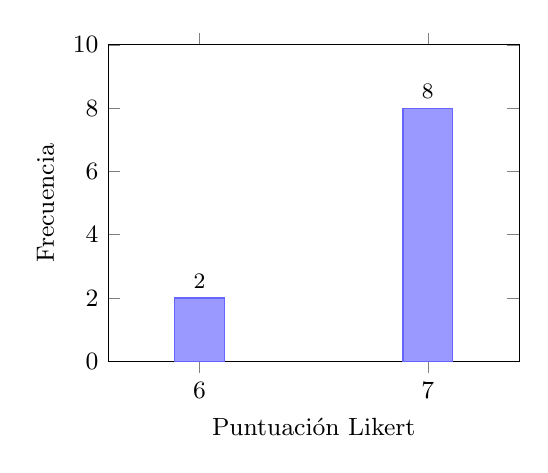
\begin{tikzpicture}
\begin{axis}[
  ybar, bar width=18pt,
  xlabel={Puntuación Likert},
  ylabel={Frecuencia},
  xtick=data,
  ytick={0,2,4,6,8,10},
  ymin=0, ymax=10,
  width=6.8cm, height=5.6cm,
  nodes near coords,
  every node near coord/.append style={font=\footnotesize},
  enlarge x limits=0.4,
  fill=blue!40,
  tick label style={font=\small},
  label style={font=\small},
]
\addplot[fill=blue!40, draw=blue!60] coordinates {(6,2) (7,8)};
\end{axis}
\end{tikzpicture}
\par\vspace{4pt}
{\small\textbf{PEOU10} — Activación modo completo\par $\bar{x}=6{,}82$;}
\end{minipage}
\hfill
\begin{minipage}[t]{0.47\linewidth}
\centering
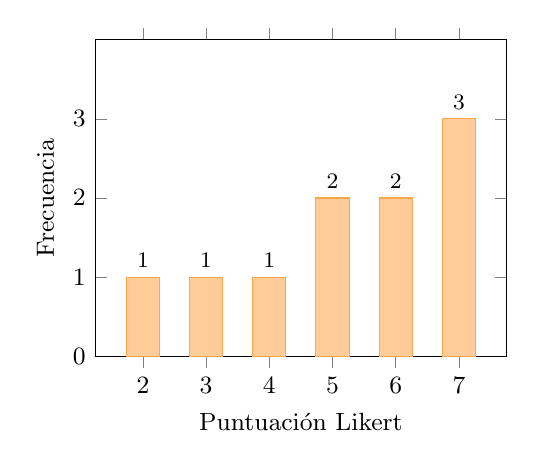
\begin{tikzpicture}
\begin{axis}[
  ybar, bar width=12pt,
  xlabel={Puntuación Likert},
  ylabel={Frecuencia},
  xtick=data,
  ytick={0,1,2,3},
  ymin=0, ymax=4,
  width=6.8cm, height=5.6cm,
  nodes near coords,
  every node near coord/.append style={font=\footnotesize},
  enlarge x limits=0.15,
  fill=orange!40,
  tick label style={font=\small},
  label style={font=\small},
]
\addplot[fill=orange!40, draw=orange!70] coordinates {(2,1) (3,1) (4,1) (5,2) (6,2) (7,3)};
\end{axis}
\end{tikzpicture}
\par\vspace{4pt}
{\small\textbf{PEOU7} — Entrada por voz\par $\bar{x}=5{,}09$;}
\end{minipage}
\caption{Distribución de respuestas para los ítems extremos del Bloque C ($n=11$): ítem de mayor puntuación (PEOU10) e ítem de menor puntuación y mayor dispersión (PEOU7).}
\label{fig:barchart-peou}
\end{figure}

%%%%%%%%%%%%%%%%%%%%%%%%%%%%%%%%%%%%%%%%%%%%%%%%%%%%%%%%%%%
\section{Intención de uso}\label{sec:resultados-itu}
%%%%%%%%%%%%%%%%%%%%%%%%%%%%%%%%%%%%%%%%%%%%%%%%%%%%%%%%%%%

La media compuesta de intención de uso (ITU) fue $\bar{x}_{\text{ITU}} = 5{,}65$ ($SD = 1{,}00$). La desviación estándar más alta de los tres constructos refleja una mayor heterogeneidad en las intenciones de uso, en parte explicable por las distintas trayectorias profesionales de los participantes. La tabla~\ref{tab:ituItems} muestra las medias por ítem.

\begin{table}[h!]
\centering
\caption{Medias por ítem del Bloque~D (Intención de uso, $n = 11$; escala 1--7).}
\label{tab:ituItems}
\begin{tabular}{@{} c p{9.5cm} c @{}}
\hline
\rule{0pt}{10pt}\textbf{Ítem} & \textbf{Enunciado resumido} & $\bar{x}$ \\
\hline
\rule{0pt}{10pt}ITU1 & Tengo intención de utilizar este sistema en el futuro & 4{,}91 \\
ITU2 & Recomendaría este sistema a compañeros que necesiten crear diagramas BPMN & 6{,}36 \\
ITU3 & Si tuviera acceso, lo utilizaría con regularidad en mi entorno de trabajo o estudio & 5{,}55 \\
ITU4 & Preferiría este sistema antes que herramientas de modelado tradicionales & 6{,}09 \\
ITU5 & Utilizaría este sistema para introducir a otras personas en el modelado BPMN & 5{,}36 \\
\hline
\multicolumn{2}{@{}l}{\rule{0pt}{10pt}\textbf{Puntuación compuesta ITU}} & \textbf{5{,}65} \\
\hline
\end{tabular}
\end{table}

El ítem con mayor puntuación es ITU2 ($\bar{x} = 6{,}36$), que refleja la disposición a recomendar el sistema: los participantes se muestran claramente proclives a prescribirlo a terceros, lo que indica una valoración global positiva. ITU1 ($\bar{x} = 4{,}91$), la intención de uso personal en el futuro, obtiene la puntuación más baja del bloque. Una posible explicación es que la mayoría de los participantes son estudiantes sin un rol profesional en BPM, de modo que la intención de uso futuro depende de su acceso continuado a contextos en los que el modelado de procesos sea necesario. Este efecto de contexto es habitual en estudios TAM con muestras académicas y no invalida la valoración positiva de utilidad y facilidad de uso.

La figura~\ref{fig:barchart-itu} muestra que ITU2 concentra 7 de 11 respuestas en el valor máximo 7, mientras que ITU1 presenta una distribución asimétrica negativa más marcada, con un participante en el valor 2 que deprime la media respecto a la moda (6).

\begin{figure}[h!]
\centering
\begin{minipage}[t]{0.47\linewidth}
\centering
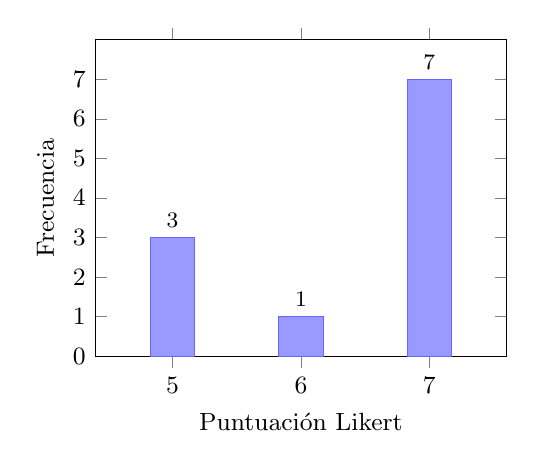
\begin{tikzpicture}
\begin{axis}[
  ybar, bar width=16pt,
  xlabel={Puntuación Likert},
  ylabel={Frecuencia},
  xtick=data,
  ytick={0,1,2,3,4,5,6,7},
  ymin=0, ymax=8,
  width=6.8cm, height=5.6cm,
  nodes near coords,
  every node near coord/.append style={font=\footnotesize},
  enlarge x limits=0.3,
  fill=blue!40,
  tick label style={font=\small},
  label style={font=\small},
]
\addplot[fill=blue!40, draw=blue!60] coordinates {(5,3) (6,1) (7,7)};
\end{axis}
\end{tikzpicture}
\par\vspace{4pt}
{\small\textbf{ITU2} — Recomendaría el sistema\par $\bar{x}=6{,}36$;}
\end{minipage}
\hfill
\begin{minipage}[t]{0.47\linewidth}
\centering
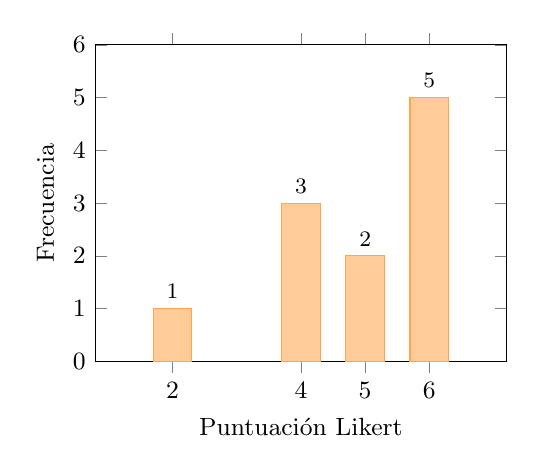
\begin{tikzpicture}
\begin{axis}[
  ybar, bar width=14pt,
  xlabel={Puntuación Likert},
  ylabel={Frecuencia},
  xtick=data,
  ytick={0,1,2,3,4,5,6},
  ymin=0, ymax=6,
  width=6.8cm, height=5.6cm,
  nodes near coords,
  every node near coord/.append style={font=\footnotesize},
  enlarge x limits=0.3,
  fill=orange!40,
  tick label style={font=\small},
  label style={font=\small},
]
\addplot[fill=orange!40, draw=orange!70] coordinates {(2,1) (4,3) (5,2) (6,5)};
\end{axis}
\end{tikzpicture}
\par\vspace{4pt}
{\small\textbf{ITU1} — Intención de uso futuro\par $\bar{x}=5{,}91$;}
\end{minipage}
\caption{Distribución de respuestas para los ítems extremos del Bloque D ($n=11$): ítem de mayor puntuación (ITU2) e ítem de menor puntuación (ITU1).}
\label{fig:barchart-itu}
\end{figure}

%%%%%%%%%%%%%%%%%%%%%%%%%%%%%%%%%%%%%%%%%%%%%%%%%%%%%%%%%%%
\section{Relaciones entre constructos}\label{sec:correlaciones}
%%%%%%%%%%%%%%%%%%%%%%%%%%%%%%%%%%%%%%%%%%%%%%%%%%%%%%%%%%%

Para examinar las relaciones entre los tres constructos TAM se calcularon los coeficientes de correlación de Pearson entre las puntuaciones compuestas de PU, PEOU e ITU. La tabla~\ref{tab:correlaciones} presenta la matriz de correlaciones.

\begin{table}[h!]
\centering
\caption{Matriz de correlaciones de Pearson entre constructos TAM ($n = 11$). \newline
* $p < {,}05$; *** $p < {,}001$ (prueba bilateral).}
\label{tab:correlaciones}
\begin{tabular}{@{} l c c c @{}}
\hline
\rule{0pt}{10pt} & \textbf{PU} & \textbf{PEOU} & \textbf{ITU} \\
\hline
\rule{0pt}{10pt}PU   & 1{,}00      & 0{,}94*** & 0{,}89*** \\
PEOU &            & 1{,}00    & 0{,}75*   \\
ITU  &            &           & 1{,}00    \\
\hline
\end{tabular}
\end{table}

Las tres correlaciones son estadísticamente significativas y de signo positivo, en plena concordancia con las predicciones del modelo TAM original~\cite{davis1989tam}:

\begin{itemize}
  \item La correlación entre PU y PEOU ($r = 0{,}94$, $p < {,}001$) indica que los participantes que perciben el sistema como fácil de usar tienden también a percibirlo como más útil, lo que refuerza el papel de la facilidad de uso como antecedente de la utilidad percibida postulado por Davis~\cite{davis1989tam}.
  \item La correlación entre PU e ITU ($r = 0{,}89$, $p < {,}001$) es la más sólida desde el punto de vista teórico: la utilidad percibida es el principal predictor de la intención de uso, y los datos apoyan esta relación con gran claridad.
  \item La correlación entre PEOU e ITU ($r = 0{,}75$, $p < {,}05$) también es significativa, si bien de menor magnitud, lo que es coherente con la literatura TAM que atribuye a la facilidad de uso un efecto indirecto sobre la intención mediado en parte por la utilidad percibida.
\end{itemize}

Estos resultados deben interpretarse teniendo en cuenta el tamaño muestral ($n = 11$): con $df = 9$, el valor crítico de Pearson para $p < {,}05$ (bilateral) es $r_{c} = 0{,}602$. Todas las correlaciones lo superan, por lo que son estadísticamente significativas, pero la amplitud de los intervalos de confianza, aconseja prudencia en la generalización. Los resultados son, no obstante, consistentes internamente y coherentes con los obtenidos en estudios TAM piloto de escala similar.

%%%%%%%%%%%%%%%%%%%%%%%%%%%%%%%%%%%%%%%%%%%%%%%%%%%%%%%%%%%
\section{Valoración de funcionalidades específicas}\label{sec:resultados-sp}
%%%%%%%%%%%%%%%%%%%%%%%%%%%%%%%%%%%%%%%%%%%%%%%%%%%%%%%%%%%

El Bloque~E del cuestionario recogió la valoración de once características concretas de la herramienta que no quedan recogidas directamente en los constructos TAM estándar. La puntuación compuesta del bloque fue $\bar{x}_{\text{SP}} = 5{,}70$ ($SD = 0{,}86$). La tabla~\ref{tab:spItems} presenta las medias por ítem.

\begin{table}[h!]
\centering
\caption{Medias por ítem del Bloque~E (funcionalidades específicas, $n = 11$; escala 1--7).}
\label{tab:spItems}
\begin{tabular}{@{} c p{9.5cm} c @{}}
\hline
\rule{0pt}{10pt}\textbf{Ítem} & \textbf{Enunciado resumido} & $\bar{x}$ \\
\hline
\rule{0pt}{10pt}SP1  & Modo paso a paso: suficiente control sobre el resultado final & 5{,}18 \\
SP2  & El sistema reduce la necesidad de conocimientos previos de BPMN & 5{,}18 \\
SP3  & El modo de generación completa es también una opción útil & 6{,}00 \\
SP4  & El análisis PERVAL aporta información útil sobre la calidad del proceso & 5{,}45 \\
SP5  & Confío en que el diagrama generado representa fielmente el proceso descrito & 6{,}00 \\
SP6  & La entrada por voz facilita la interacción respecto a la escritura & 5{,}00 \\
SP7  & La edición conversacional es una forma cómoda de refinar el proceso & 5{,}64 \\
SP8  & El soporte multilingüe es útil para trabajar con equipos en ambos idiomas & 6{,}09 \\
SP9  & La edición sobre el lienzo bpmn.io complementa bien la interacción conversacional & 6{,}27 \\
SP10 & Integrar el análisis PERVAL dentro de la propia herramienta es una ventaja significativa & 5{,}73 \\
SP11 & El sistema en conjunto es una solución completa para el modelado orientado al valor & 6{,}18 \\
\hline
\multicolumn{2}{@{}l}{\rule{0pt}{10pt}\textbf{Puntuación compuesta Bloque~E}} & \textbf{5{,}70} \\
\hline
\end{tabular}
\end{table}

El ítem de mayor puntuación es SP9 ($\bar{x} = 6{,}27$), que refleja que la combinación de interacción conversacional y edición directa sobre bpmn.io se percibe como una propuesta de valor coherente. SP3 y SP5 alcanzan ambos $\bar{x} = 6{,}00$: SP3 (modo de generación completa como opción útil) recibe apoyo explícito de P11  y SP5 confirma que los participantes confían en la fidelidad del diagrama generado a pesar de los errores esporádicos del LLM.

El ítem SP6 (entrada por voz, $\bar{x} = 5{,}00$) obtiene la puntuación más baja del bloque, en línea con el ítem PEOU7 de facilidad de uso. La funcionalidad de voz es valorada positivamente como concepto, pero su utilidad práctica se ve condicionada por factores de entorno (ruido, privacidad) que los participantes señalan implícitamente. SP1 y SP2 comparten la segunda posición más baja ($\bar{x} = 5{,}18$): SP2 (reducción de la necesidad de conocimientos previos de BPMN) muestra la mayor variabilidad del bloque, con respuestas que van de 1 a 7, lo que refleja la diferencia de percepción entre expertos en BPMN que ven la herramienta como complementaria y usuarios menos expertos que la valoran como democratizadora.


La figura~\ref{fig:barchart-sp2} muestra la distribución de SP2, cuya alta dispersión refleja la diferencia de criterio entre participantes con distinto nivel de expertise en BPMN. Con $n=11$, la moda sigue siendo 7 (cuatro participantes), pero los valores bajos (1 y 3) mantienen su efecto depresor sobre la media.

\begin{figure}[H]
\centering
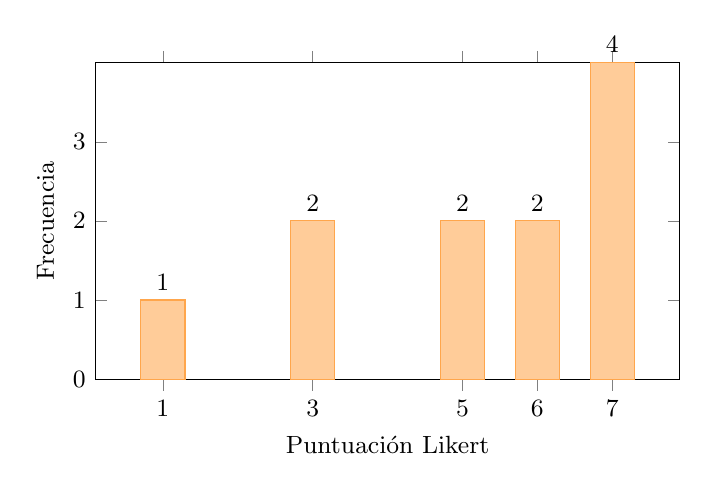
\begin{tikzpicture}
\begin{axis}[
  ybar, bar width=16pt,
  xlabel={Puntuación Likert},
  ylabel={Frecuencia},
  xtick=data,
  ytick={0,1,2,3},
  ymin=0, ymax=4,
  width=9cm, height=5.6cm,
  nodes near coords,
  every node near coord/.append style={font=\small},
  enlarge x limits=0.15,
  fill=orange!40,
  tick label style={font=\small},
  label style={font=\small},
]
\addplot[fill=orange!40, draw=orange!70] coordinates {(1,1) (3,2) (5,2) (6,2) (7,4)};
\end{axis}
\end{tikzpicture}
\caption{Distribución de respuestas del ítem SP2 \emph{«El sistema reduce la necesidad de conocimientos previos de BPMN»} ($n=11$;\; $\bar{x}=5{,}18$;\; $Mdn=6$;\; $Mo=7$). La alta dispersión refleja diferencias de criterio según el nivel de expertise previo en BPMN.}
\label{fig:barchart-sp2}
\end{figure}

%%%%%%%%%%%%%%%%%%%%%%%%%%%%%%%%%%%%%%%%%%%%%%%%%%%%%%%%%%%
\section{Análisis cualitativo de las preguntas abiertas}\label{sec:cualitativo}
%%%%%%%%%%%%%%%%%%%%%%%%%%%%%%%%%%%%%%%%%%%%%%%%%%%%%%%%%%%

El cuestionario incluía dos preguntas abiertas: (Q1)~«¿Qué funcionalidad de la herramienta te ha parecido más útil o innovadora?» y (Q2)~«¿Qué aspecto mejorarías o echarías en falta?». Las respuestas fueron codificadas temáticamente mediante análisis de contenido inductivo. Se identificaron cuatro categorías principales en Q1 y cuatro en Q2.

\subsection{Funcionalidades más valoradas (Q1)}\label{subsec:q1}

\paragraph{Generación paso a paso.} Es la funcionalidad más citada como innovadora, mencionada explícitamente por cuatro de los diez participantes (P1, P3, P7, P9). Los participantes destacan que la interacción guiada les proporciona un grado de control sobre el resultado que no encuentran en sistemas de generación autónoma. P7 lo sintetiza con precisión: \textit{«la generación paso a paso [...] resulta un punto de encuentro muy interesante entre el uso de IA y el mantenimiento del control por parte del usuario»}.

\paragraph{Generación mediante lenguaje natural.} Cinco participantes (P4, P6, P9, P10, P11) destacan la capacidad de describir el proceso en lenguaje natural como la característica más innovadora, con independencia del modo de generación utilizado. P9 señala que \textit{«la opción de poder crear diagramas BPMN con lenguaje natural me parece muy útil e innovadora ya que puede reducir la carga de trabajo»}. P10 añade el valor de la organización automática del lienzo: \textit{«facilita mucho la creación de diagramas BPMN, al organizar todo en el espacio por ti»}.

\paragraph{Integración del análisis PERVAL.} P2 destaca conjuntamente la generación automática y el análisis PERVAL, valorando que este último \textit{«añade una valoración adicional al diagrama y ayuda a identificar los puntos que aportan más valor al usuario»}.

\paragraph{Velocidad y accesibilidad.} P8 señala como principal ventaja la \textit{«velocidad y sencillez sin necesidad de tener altos conocimientos previos en BPMN»}, perspectiva coherente con su valoración de SP2 y con el objetivo de democratización del modelado de procesos que motivó el diseño de la herramienta (capítulo~\ref{cap:validacion}).

\subsection{Aspectos de mejora (Q2)}\label{subsec:q2}

\paragraph{Personalización visual.} Dos participantes (P1 y P6) señalan la ausencia de control estético como la principal carencia: colores, fuentes e iconos para personalizar los elementos del diagrama. Esta funcionalidad no forma parte del alcance definido en el análisis de requisitos, que priorizó la corrección estructural del BPMN generado, pero su recurrencia en las respuestas sugiere que podría considerarse en iteraciones futuras.

\paragraph{Interfaz de usuario.} Tres participantes identifican mejoras en la interfaz: P2 señala que el panel lateral es estrecho para leer respuestas largas y solicita zoom automático sobre el diagrama generado; P9 apunta que la interfaz \textit{«es bastante simple»} y que la IA \textit{«comete algunos errores que necesitan ser corregidos»}; P10 solicita mejoras de legibilidad y accesibilidad.

\paragraph{Edición híbrida.} P5 y P8 indican que les gustaría poder editar el diagrama manualmente sobre el lienzo y que el agente conversacional reconozca y continúe asistiendo a partir de ese estado modificado. P8 describe el comportamiento actual: \textit{«al editarlo a mano a mitad del proceso, el agente da por terminado el diagrama y no continua asistiendo»}. Esto refleja una limitación técnica de la arquitectura actual: el estado del XML en el cliente y el contexto de la conversación en el servidor MCP no están sincronizados cuando el usuario modifica el lienzo directamente.

\paragraph{Incorporación al flujo de trabajo.} P4 solicita un tutorial inicial con explicación de los elementos de la interfaz y una leyenda de notación BPMN para usuarios no expertos. P7 coincide en que la primera vez que se accede a la herramienta la curva de aprendizaje no es del todo intuitiva, si bien valora positivamente la experiencia una vez familiarizado.

\paragraph{Corrección de errores en refinamiento conversacional.} P5 reporta un comportamiento defectuoso observado durante las sesiones de evaluación: \textit{«cuando le pido al asistente varias modificaciones seguidas, a veces hace los cambios que le indico, pero vuelve a una versión anterior del diagrama»}. Este comportamiento es coherente con la limitación de los modelos LLM para mantener el estado acumulado del XML a lo largo de múltiples turnos de edición conversacional, e ilustra una amenaza a la validez interna identificada en el capítulo~\ref{cap:validacion}.

%%%%%%%%%%%%%%%%%%%%%%%%%%%%%%%%%%%%%%%%%%%%%%%%%%%%%%%%%%%
\section{Discusión de resultados}\label{sec:discusion-resultados}
%%%%%%%%%%%%%%%%%%%%%%%%%%%%%%%%%%%%%%%%%%%%%%%%%%%%%%%%%%%

Los resultados del estudio permiten responder afirmativamente a la pregunta de validación planteada en el capítulo~\ref{cap:validacion}: los usuarios del perfil objetivo perciben la herramienta como útil, fácil de usar y tienen intención de recomendarla y utilizarla en contextos futuros.

Las puntuaciones compuestas de los tres constructos TAM superan el valor de referencia de $6{,}0$ sobre $7$ para PU ($\bar{x}=6{,}19$) y PEOU ($\bar{x}=6{,}17$), y de $5{,}5$ para ITU ($\bar{x}=5{,}65$), lo que sitúa la herramienta en la región de aceptación tecnológica positiva. Las correlaciones inter-constructo, todas significativas ($r \in [0{,}75,\, 0{,}94]$), reproducen la estructura factorial del TAM original~\cite{davis1989tam} y el patrón típico de estudios de aceptación de herramientas asistidas por IA: la utilidad percibida es el predictor más fuerte de la intención de uso, y la facilidad de uso actúa como antecedente de la utilidad. La consistencia interna de las tres escalas ($\alpha = 0{,}87$) descarta problemas de fiabilidad del instrumento.

Dos contribuciones del diseño de la herramienta reciben un respaldo empírico especialmente claro. En primer lugar, el modo de generación guiada paso a paso es consistentemente identificado como la característica más innovadora por P1, P3, P7 y P9, mientras que P11 destaca el modo de generación completa como punto de partida preferido. Esta divergencia de criterio refleja perfiles de usuario distintos: quienes valoran el control prefieren la generación paso a paso, mientras que quienes priorizan la velocidad y la visión global prefieren la generación completa. Ambos modos reciben valoraciones positivas (PU7 $= 5{,}82$, PU10 $= 6{,}64$). En segundo lugar, la confianza en la fidelidad del diagrama generado (SP5, $\bar{x} = 6{,}00$) se mantiene alta pese a los errores esporádicos del LLM, lo que sugiere que el mecanismo de validación explícita en cada paso actúa como salvaguarda suficiente para los usuarios.

Entre las limitaciones del estudio, el tamaño muestral ($n = 11$) es la más relevante para la interpretación estadística. Los resultados deben considerarse indicativos del comportamiento de la herramienta con usuarios del perfil evaluado, no generalizables sin una replicación con muestra mayor. El sesgo de familiaridad con IA (el $63,6$\,\% de los participantes usa IA generativa diariamente) puede también haber favorecido las valoraciones de facilidad de uso respecto a lo que cabría esperar en una muestra de usuarios de BPMN sin experiencia en IA.

Las observaciones cualitativas señalan cuatro líneas de trabajo futuro para incrementar la aceptación de la herramienta: (i)~mejorar la sincronización entre el estado del lienzo bpmn.io y el contexto conversacional del agente para permitir la edición híbrida; (ii)~añadir un tutorial de incorporación (\textit{onboarding}) que reduzca la curva de aprendizaje inicial; (iii)~explorar la personalización visual del diagrama como característica opcional; y (iv)~incorporar mecanismos de explicabilidad que permitan al sistema justificar las decisiones de modelado y responder preguntas sobre el diagrama generado en lenguaje natural conversacional.

%%%%%%%%%%%%%%%%%%%%%%%%%%%%%%%%%%%%%%%%%%%%%%%%%%%%%%%%%%%
%% Final del capítulo de resultados
%%%%%%%%%%%%%%%%%%%%%%%%%%%%%%%%%%%%%%%%%%%%%%%%%%%%%%%%%%%
